% Replaces main.tex Section 3.1. Reserve Proposition 1 for Appendix A.
\subsection{Utility mismatch under ratio risk}
Let $X$ be the information available when acceptance is chosen. For
nonnegative integrable loss $L$ and exposure $W$, define
\[
 \ell(X)=\E[L\mid X],\quad w(X)=\E[W\mid X],\quad T=\E W>0,
 \quad a(X)\in[0,1].
\]
Row coverage, exposure coverage, and accepted ratio risk are
\begin{equation}
 c(a)=\E a,\qquad d_W(a)=\frac{\E[aW]}{T},\qquad
 R(a)=\frac{\E[aL]}{\E[aW]}.
 \label{eq:ratio}
\end{equation}
The accepted denominator must be positive. The acceptance constraint is $R(a)\leq r$
and $c(a)\geq c_0$. Its signed excess is
\begin{equation}
 g_r=L-rW,\qquad m_r=\ell-rw,\qquad
 R(a)\leq r\ \Longleftrightarrow\ \E[a m_r]\leq0.
 \label{eq:excess}
\end{equation}
WAPE is the specialization $L=|Y-f(X)|$, $W=Y$, with $Y,f\geq0$;
then $\ell=e$, $w=\mu$, and $d_W=d$ is demand coverage.

Fixed-row-coverage excess is minimized by accepting the smallest
$m_r$ values, with randomization on ties (Proposition~\ref{prop:threshold}
in Appendix~\ref{app:proofs}). To maximize exposure instead, change measure
to $d\nu=w\,dP_X/T$ after rejecting $w=0,\ell>0$ contexts: then $d_W(a)=\E_\nu a$ and
$R(a)=\E_\nu[a\ell/w]/\E_\nu a$.
\setcounter{proposition}{1}
\begin{proposition}[Exposure-weighted ranking]
\label{prop:weighted}
If a positive-exposure feasible rule exists and the row floor is
nonbinding, exposure coverage is optimized by thresholding $\ell/w$,
with boundary randomization. Reject $w=0,\ell>0$ contexts; $w=\ell=0$
contexts are neutral for this objective. The ranking is independent of
$r$; its threshold is not.
\end{proposition}
Thus the population rankings are $\ell-rw$ for rows and $\ell/w$ for
exposure. A fixed ranking's largest feasible threshold maximizes either
coverage because its acceptance sets are nested; objective comparisons
must therefore also compare ranking families (Appendix~\ref{app:objective}).

For disjoint context sets $K,U$, write
\[
 M_A=\E[\ind_Aw],\qquad B=-\E[\ind_Km_r],\qquad
 M_K>0,\quad B\geq0.
\]
Here $B$ is the excess slack supplied by a common accepted set.
\begin{proposition}[Sharp objective reversal for ratio risk]
\label{prop:lowdemand}
Fix $r>0$, $\rho>r$, and $\varepsilon>0$. If $\ell=\rho w$ on $U$ and
$0<M_U\leq\varepsilon\Pr(U)$, then $R(\ind_U)=\rho$ and
$K\cup U$ satisfies the cap exactly when $(\rho-r)M_U\leq B$.
Accepting $U$ adds $\Pr(U)$ row coverage but at most
$\varepsilon\Pr(U)/T$ exposure coverage.

For every $0\leq c_0<1$ and $\eta>0$, there exists a three-context
law with $w>0$, $0\leq\ell\leq\rho w$, and exact conditional moments
whose unique row- and exposure-optimal policies $a_R,a_W$ satisfy
the cap and the nonbinding row floor, and obey
\[
 c(a_R)-c(a_W)>1-c_0-\eta,\qquad
 d_W(a_W)-d_W(a_R)>1-\eta.
\]
The universal bounds $1-c_0$ and $1$ are jointly sharp. For
$0<r<1$ and $\rho=1$, this sharpness also holds with binary $0\leq L\leq W\leq1$.
\end{proposition}
Approaching the joint bounds uses a sequence with vanishing conditional exposure; the construction does not establish typical or nondegenerate empirical gaps. The sharpness statement ranges over joint laws that can realize the
conditional moments in Appendix~\ref{app:proofs}; it is not a claim
about every fixed metric class. If $W$ is constant, for example,
$d_W=c$ and reversal is impossible. For a fixed multi-label classifier, whole-example abstention yields an exact micro-precision reversal (Appendix~\ref{app:classification}). Ordinary binary precision with an unrestricted gate instead has a common optimum for both coverage objectives. For whole-example micro-precision with $1\leq w\leq m$, each coverage gap is at most $(m-1)/(m+1)$; Appendix~\ref{app:bounded_exposure} sharpens this to a joint bound.

\paragraph{When reversal is limited or absent.}
For row- and exposure-optimal policies on a common feasible set, let
$x=c(a_R)-c(a_W)\geq0$ and $y=d_W(a_W)-d_W(a_R)\geq0$.
If $0<u\leq w\leq v$, then, with $D=(v-u)/(v+u)$,
\begin{equation}
 y\leq\frac{D-x}{1-Dx},\qquad 0\leq x,y\leq D.
 \label{eq:bounded}
\end{equation}
Thus constant positive conditional exposure rules out reversal. Moreover,
with unrestricted randomized acceptance under just the pooled risk cap and row
floor, at most two positive-probability, positive-exposure contexts have a common
optimum whenever feasible. Strict reversal requires at least three such contexts.
Appendix~\ref{app:bounded_exposure} proves both claims; variation alone is not
sufficient, as $\ell\equiv0$ makes accept-all optimal for any exposure.

\paragraph{WAPE corollary and estimation.}
For $0<r<1$, setting $\rho=1$, $W=Y$, and $f=0$ on $U$ gives
$e=\mu$: near-zero-demand rows have budget cost $(1-r)\mu$ yet
unit row reward. The three-context law is realizable by deterministic
nonnegative forecasts (Appendix~\ref{app:proofs}), so both sharp bounds
hold for WAPE. A low-exposure share alone cannot bound the forgone
exposure without a positive excess-rate margin; the appendix gives
that bound and the exact budget identity. More generally $|e-\mu|\leq f$.
Exact-head optimality does not imply estimated-ratio robustness.
Section~\ref{sec:objectives} and Appendix~\ref{app:proofs} distinguish
objective alignment from small-denominator error amplification.

\paragraph{From head error to decision error.}
Small head error alone does not ensure small coverage regret: Appendix~\ref{app:plugin-v12} gives a two-context example with vanishing error and a limiting $1/2$ coverage loss. A conditional perturbation bound controls coverage and risk when a strictly feasible comparator and positive accepted exposure exist. This specializes established constraint-sensitivity arguments; its assumptions do not certify the fitted menu.

\subsection{A fixed classifier: examples versus positive predictions}
\label{sec:classification}
Consider a fixed two-label classifier with whole-example abstention. Exposure $W$ counts its positive predictions, and loss $L$ counts false positives, so $1-R$ is accepted micro-precision. Three contexts have the following known conditional moments:
\[
\begin{array}{c|ccc}
 &K&U&V\\\hline
 \Pr(X)&2/5&2/5&1/5\\
 h(X)&(1,0)&(1,0)&(1,1)\\
 w(X)&1&1&2\\
 \ell(X)&0&3/10&1/2
\end{array}
\]
At risk cap $r=1/10$ and case floor $c_0=7/20$, every optimum accepts $K$. Its risk surplus funds the remaining constraint $4a_U+3a_V\leq2$. Maximizing accepted examples chooses $(a_K,a_U,a_V)=(1,1/2,0)$, giving $(c,d_W)=(3/5,1/2)$. Maximizing accepted positive predictions instead chooses $(1,0,2/3)$, giving $(8/15,5/9)$. Both attain exactly 90\% micro-precision. The classifier is unchanged; only the value assigned to acceptance differs (Figure~\ref{fig:mechanism}). Appendix~\ref{app:classification} specifies the label distribution and verifies both optima.

For ordinary binary precision, accepting all predicted-negative cases costs no risk budget, and completed gates satisfy $c=1-T+Td_W$. Both objectives then have a common optimum. This contrast makes the acceptance unit consequential: gating each label separately would change the multi-label problem above.

\begin{figure}[t]
\centering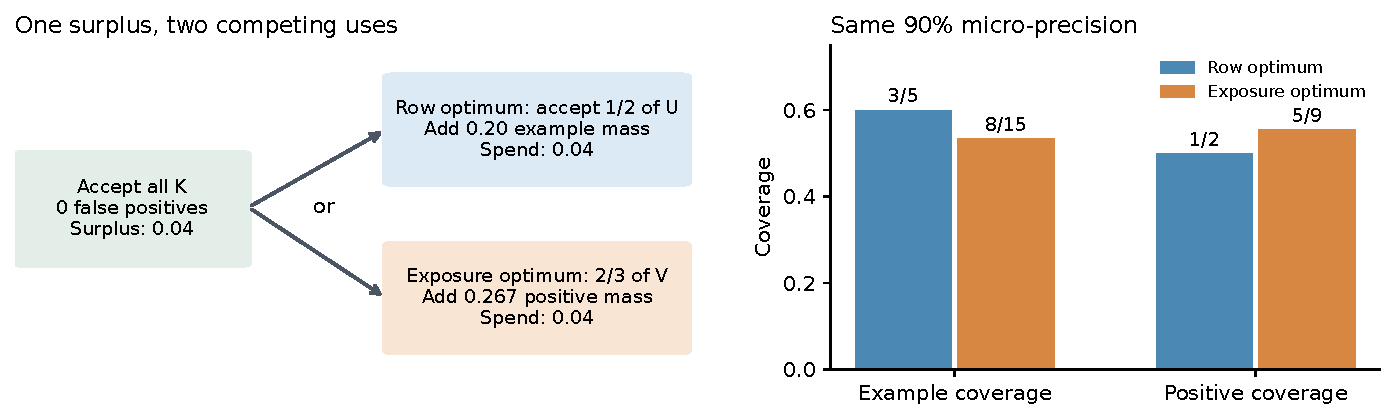
\includegraphics[width=\linewidth]{figures/utility_mechanism.pdf}
\caption{Exact fixed-classifier example, not an empirical benchmark. Left: the accurate context $K$ supplies 0.04 expected excess units; either competing allocation uses all of them. Right: the same risk budget buys more examples or more positive predictions, but not both. Fractional acceptance is independent randomization within a context.}
\label{fig:mechanism}
\end{figure}

